\ifpdf
    \graphicspath{{Chapter_2006/figures/PNG/}{Chapter_2006/figures/PDF/}{Chapter_2006/figures/}}
\else
    \graphicspath{{Chapter_2006/figures/EPS/}{Chapter_2006/figures/}}
\fi

\section{Discussion}\label{sec:2006/discussion}

\subsection{Tracer relations}\label{ssec:2006/discuss/tracer}

The relationship between ozone and carbon monoxide (\chem{CO}) has been used to study tropospheric-stratospheric transition in
chemical regimes \citep[e.g.][and references therein]{Pan:2007sw,Hegglin:2009fk}. Similarly, it may be applied to tropospheric data
alone to identify contributions from various pathways \citep[e.g.][]{Zhang:2006zr,Voulgarakis:2011fk,Cristofanelli:2013uq}. Ignoring
\chem{NO_x}, ozone is expected to be strongly positively correlated with \chem{CO} \citep{Chin:1994kx}. However, since the dominating
source for \chem{CO} is surface emission, with a limited lifetime, \chem{CO} decreases rapidly with height. At the same time, significant
contribution of stratospheric ozone and upper tropospheric production cause ozone to increase rapidly with height. Together, \chem{O_3-CO}
correlation over a sufficiently expansive column can expect to observe an "L"-shaped joint distribution.

\figuremacroN{tracer/tracer_correlations}{\chem{CO}-\chem{O_3} model correlation}{\label{fig:2006/o3co}
\textbf{(a)} Anticyclone ($\bar{Z}_{300}>9730\,\unit{m}$) \chem{CO}-\chem{O_3}(adjusted) joint-distribution separately
colored by pressure levels. \textbf{(b)} Same as \textbf{a} but outside the anticyclone between 9710\,\unit{m} and
9730\,\unit{m}. Data points south of 25$^\circ$N have been removed to reduce impact of the southern boundary. \vspace{-.2in}}

Here we correlated the August average model ozone and \chem{CO} from the surface up to 100\,\unit{hPa} (Fig.~\ref{fig:2006/o3co}.
Data points are first separated by within and outside of the anticyclone, defined by the boundary $\bar{Z}_{300}$ as previously
defined in Section~\ref{ssec:2006/gen/ozone}. Then, each panel is further classified by pressure level split at 300 and 700\,\unit{hPa}
to represent the lower, middle, and upper troposphere. To account for model biases, ozone VMRs between 100--300\,\unit{hPa}
have been adjusted by the differences in mean and variance against TES computed in Section~\ref{ssec:2006/gen/ozone}. No
adjustment is performed at the other pressure levels due to insignificant bias compared to observations. While the value shifted,
the shape and features of the joint-distribution remain consistent before and after the adjustment. The labeled features annotated
in the figure are discussed below.

Feature A indicates a type of air mass exist only outside the anticyclone. This unique feature corresponds to subtropical Atlantic
influx from the southern boundary. Typically, it has higher \chem{CO} but the ozone VMRs at 300\,\unit{hPa} from lower latitudes are
lower in general. These air masses intermittently contribute to the anticyclone, similar to the air masses mixed across the jet stream
from the north (see Sect.~\ref{ssec:2006/gen/ozone} \& \ref{ssec:2006/gen/co}). Feature B indicates the upper tropospheric branch
of the \chem{O_3}-\chem{CO} correlation. It is evident from the labels, which are placed at the same locations in both panels, that
\chem{CO} is more effective in raising the ozone level within the upper troposphere above the baseline, indicated by the dashed
line (feature C). Similar to the alphabetic labels, the baseline is also identical in both panels. Thus, it can be seen that the background
\chem{O_3}-\chem{CO} correlations are consistent both inside and outside the anticyclone. Finally, feature D denotes the mid-to-lower
tropospheric branch, which includes the boundary layer. Similar to B, D is chemically different across the anticyclone. Since circulation
is not a factor at low altitudes, the other plausible explanation is the abundant sources of anthropogenic and biogenic emissions of both
VOCs and \chem{NO_x}, which subsequently enhance in-situ ozone production within this layer and transported upwards. Finally,
The low-\chem{CO}, low-\chem{O_3}  value at the interface of lower and middle tropospheres is about 10\,\unit{ppbv} higher within
the anticyclone compared to the $\sim38$\,\unit{ppbv} value outside of the region despite negligible differences in their corresponding
\chem{CO} level.

The analysis above shows that the condition within the anticyclone enables higher ozone values throughout the entire troposphere at
a wide range of VMRs for \chem{CO} (features B and C). Since emission dominates transport in the lower
troposphere, the appropriate hypothesis for the enhancement at C is the elevated level of \chem{NO_x} from either co-located
emissions or subsidence of {\lnox} within the region. However, more information is required to properly diagnose feature B, which
can be either an indication of enhanced \chem{O_3} chemical production at the 80\,\unit{ppbv} \chem{CO} or enhanced \chem{CO}
at levels with \chem{O_3} through convective detrainments.

\figuremacroW{tracer/tracer_maps}{Passive tracers}{\label{fig:2006/tracers}
First row ({\bf a,b}) shows the August average of lateral boundary decaying tracer at 300\,\unit{hPa} on the left and along
33$^\circ$N on the right. Values are given in percentage. Second row ({\bf c,d}) shows the surface layer deacying tracer.
Third row ({\bf e,f}) shows the stratospheric decaying tracer.
Last row ({\bf g,h}) shows the lightning decaying tracer given in \unit{ppbv}.}{0.9}

Figure~\ref{fig:2006/tracers} shows four of the tracers released from the lateral boundaries, the boundary layer, the stratosphere, and
lightning sources. All tracers shown are the decaying type with a lifetime of 1 day (1-d). The impact of the NAM circulation is clearly shown
in the spatial distribution of the lateral boundary (BC) tracer (Fig.~\ref{fig:2006/tracers}{\bf a}). Within the anticyclone region ($\bar{Z}_{300}
>9730\,\unit{m}$), air mass retains no more than an average of 3\% of the characteristics from any of the boundaries. Since these
tracers are dynamically-driven, it can be asserted that the impact of boundary condition on the principle results will be minor.

Similarly, lightning (LT) tracer also shows substantial localized enhancement within the anticyclone region (Fig.~\ref{fig:2006/tracers}{\bf g}).
The observed eastward shift from the 9730\,\unit{m} contour can be explained by the overall higher lightning flash rate in the southeastern 
United States. Accounting for the one order of magnitude deviation from observed CG flash rate, the maximum accumulated lightning
1-d tracer is 0.5\,\unit{ppbv}. Despite a fixed maximum emission altitude of 6--8\,\unit{km} ($\sim400\,\unit{hPa}$) according to
\citet{Ott:2010lo}, vertical distribution along the 33$^\circ$N cross-section shows that the tracer has values $>3\,\unit{ppbv}$ (0.3
after account for overprediction in flash rate) within a wide range of pressure levels between 120--500\,\unit{hPa}
(Fig.~\ref{fig:2006/tracers}{\bf h}). Finally, the abundance of lightning tracers in the stratosphere is likely the direct result of using a
fixed altitude-dependent emission profile, which includes more than 10\% (35\,\unit{moles\,flash^{-1}}) above 12\,\unit{km} for
subtropical latitudes.

However, the spatial distribution of boundary layer (BL) tracer shows little correlation with the shape or positioning of the anticyclone. Instead,
the features of the tracer at 300\,\unit{hPa} are dominated by orographic influence of the Rocky Mountains (Fig.~\ref{fig:2006/tracers}{\bf c}).
Similarly, stratospheric (ST) tracer also shows very minimal impact from the NAM circulation except for the influx of stratospheric air eddy
shedding across the jet stream in the outflow region along the eastern seaboard.

\figuremacroW{tracer/age_maps}{Passive tracer age}{\label{fig:2006/tracer_age}
Same as Figure~\ref{fig:2006/tracers} except for tracer equivalent age. Darker colored regions represent young tracers, while lighter
colored/white regions represent aged tracers}{0.9}

The tracer equivalent age, calculated according to Equation~\ref{eqn:tracer-age}, is mapped in Figure~\ref{fig:2006/tracer_age}.
Similar to the decaying tracer distributions, BC and LT tracers are the only ones showing some correlations with the anticyclone boundary.
The range of age for BC tracer within the anticyclone is 2.6--6.8 days while the range outside the anticyclone between 9710\,\unit{m} and
9730\,\unit{m} is 1.5--4.8 days. On the contrary, LT tracer age ranges from 10.9--21.8\,\unit{hrs} within the anticyclone and 13.1--22.5\,\unit{hrs}
just outside. The primary contribution to the LT distribution is that the anticyclone encompasses areas with high lightning flash frequencies,
and thus younger tracers are expected only on the eastern $\sim2/3$ of the anticyclone as well as towards the outflow region along
the East Coast. On the west end of the cross-section (Fig.~\ref{fig:2006/tracer_age}{\bf h}), the upper tropospheric presence of LT tracer
(Fig.~\ref{fig:2006/tracers}{\bf h}) is shown to be disconnected from the high LT tracer core within the anticyclone.

\figuremacroN{tracer/passive_correlations}{BL-ST tracer correlation}{\label{fig:2006/blst}
Same as Fig.~\ref{fig:2006/o3co} but for BL and ST decaying tracers. \vspace{-.2in}}

Individually, BL and ST are dominated by orographic or large scale features. By correlating the two tracers, differences emerge.
Figure~\ref{fig:2006/blst} shows the joint distribution between the two decaying tracers. At feature A, or absence thereof within the
anticyclone, low ST-low BL data points exist only in the mid-troposphere (300--700\,\unit{hPa}) outside the anticyclone. Similarly,
feature C (moderate ST/BL) occurs outside the anticyclone only. These two features point to higher heterogeneity of air mass sourcing
outside the anticyclone than within the anticyclone between 700 and slightly above 300\,\unit{hPa}. Such result can be attributed to
the geographic diversity outside the anticyclone, primarily the presence of marine surfaces. Finally, both regions show very little
differences close to the tropopause, where ST$\sim1$.

The result in this section partially contradicts that of \citet{Li:2005ss} and \citet{Cooper:2007cr}, in particular, the conjecture that the anticyclone
enables higher ozone production through recirculation and entrapment of detrained BL air rich in ozone chemical precursors. The result here
shows that the vertical colocation of geographical homogeneity as well as meteorological factors (e.g. high lightning intensity) are the key factors
driving the ozone enhancement. On the other hand, the lack of model lateral boundary influence, as indicative of the BC tracer low within the
anticyclone, points to low externality as a secondary factor as opposed to internal conditioning. The only\footnote{Even though the simulation used
in this study does not have aircraft emissions, it can be conjectured that the influence of aircraft emission on upper tropospheric ozone production
may also be enhanced by the transport pattern due to the emission altitude and $x$-$y$ spatial distribution being similar to {\lnox}.}exception to
the irrelevance of internal condition is the influence from lightning emissions, which shows correlation with the transport pattern of the anticyclone.

\subsection{Tendency diagnostics}\label{ssec:2006/discuss/tendency}

The changes in the mixing ratio of a chemical species at a specific time and location, or tendency, can be expressed as
the sum of following components: chemistry, convection, vertical mixing, horizontal advection, vertical advection, emission,
and other loss rates (Eq.~\ref{eqn:tendency}). In the upper troposphere, except for \chem{NO}, both emissions and other
uncharacterized loss rates should be zero, and thus the total tendency can be expressed solely by the first five processes.
Consequently, inference of chemical and dynamical structures of the ozone budget is possible using these diagnostics.
Tendency diagnostics of these 5 components are available for \chem{O_3}, \chem{CO}, \chem{NO}, \chem{NO_2}, \chem{HO}
\chem{HO_2}, \chem{TOL}, and \chem{HC5} in WRF-Chem.\footnote{TOL$=$Toluene; HC5$=$Bulk species for alkane with moderate \chem{HO}
rate constants. These replace isoprene and \chem{HNO_3} in the default implementation.}

	\begin{wrapfigure}{o}{0.5\textwidth}
		\centering
		\begin{singlespacing}
		\vspace{-.2in}
		\label{fig:2006/tend_residual}
		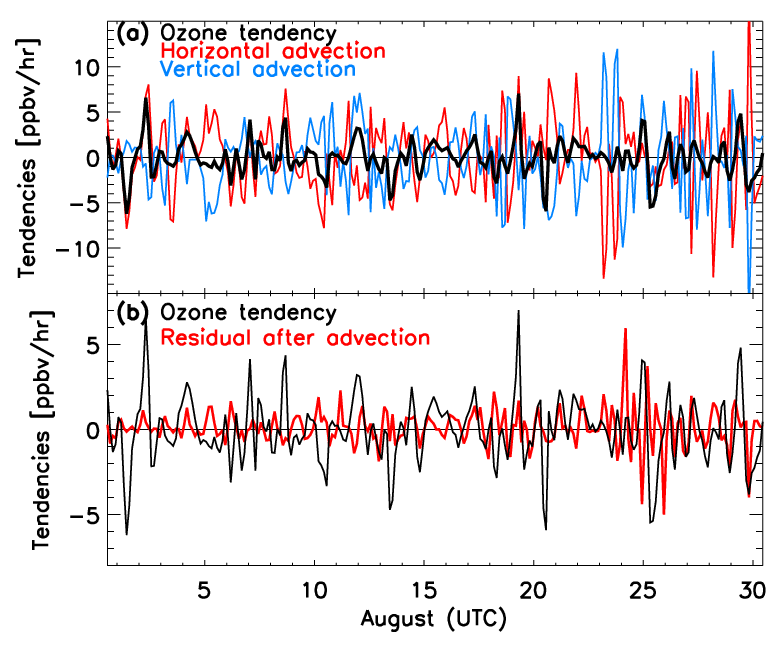
\includegraphics[width=0.48\textwidth]{tendency/residual}
		\caption[Ozone advective tendency]{{\small\textbf{Ozone advective tendency} --- Ozone tendencies and ({\bf a}) advective tendencies
		and ({\bf b}) residual tendencies after removing advections between 200--600\,\unit{hPa}. \vspace{-.2in}}}
		\end{singlespacing}
	\end{wrapfigure}

\figuremacroW{tendency/timeseries.png}{Time series for upper tropospheric tendency diagnostics}{\label{fig:2006/tendency_timeseries}
Time series at ({\bf a}) Trinidata Head, ({\bf b}) Houston, and ({\bf c}) Beltsville showing the min-mean-max ozone time series (black)
between 270--330\,\unit{hPa} overlaid with IONS-06 ozonesonde measurements represented as red vertical lines for the range and solid
$\diamondsuit$ for the mean value. Lightning \chem{NO_x} 1-d tracer (cyan) and ozone chemical (red), convective (blue), and vertical
mixing (purple) tendency components are given according to the blue axis labels on the right in units of \unit{ppbv/3\,hr}. Boundary layer (BL, blue)
and stratospheric (ST, red) are also given in \unit{\%}.}{0.9}

The primary sources for local temporal variabilities are horizontal and vertical advections. Figure~\ref{fig:2006/tend_residual} shows
the advective tendencies for ozone compared to the total ozone tendency sampled near Houston between 200--600\,\unit{hPa}.
Both the horizontal and vertical components are often on the same magnitude as the total tendency. However, the combined
advective tendency is frequently much smaller because the two components are often anti-correlated with opposite signs. The residual
tendency, i.e. the total ozone tendency without the two advective components, can be accounted for by chemical, convective, and
vertical mixing tendencies. It is useful to note that the residual is not guaranteed to be smaller than the total tendency due to the ability for advective tendencies
to ``cancel'' out the effect of the remaining three components, as seen after August 23.

To characterize the residual tendency of the continental inflow, the anticyclone, and the continental outflow, three locations are selected to be
examined further: Trinidad Head, California (40.80$^\circ$N, 124.15$^\circ$W), Houston, Texas (29.72$^\circ$N, 95.30$^\circ$W),
and Beltsville, Maryland (39.04$^\circ$N,76.52$^\circ$W). Figure~\ref{fig:2006/tendency_timeseries} shows the time series of the
ozone VMRs at these locations as well as the associated chemical, convective, and mixing tendencies. Values shown are the mean values for
all data points between 270--330\,\unit{hPa}, with min/max also indicated for ozone VMR.
To account for the model bias, IONS-06 ozonesonde measurements, described in Section~\ref{ssec:2006/gen/ozone}, are also included.
Boundary layer (BL), stratospheric (ST) and lightning (\lnox) decaying tracers, described in Section~\ref{ssec:2006/discuss/tracer}
are included to provide context of the sources for dynamical and chemical variabilities.

Trinidad Head periodically receives stratospheric ozone from the jet stream, which is responsible for the sharp spatiotemporal gradients
high VMRs simulated for particular days (e.g. August 2 and August 7). The largest 3-hourly chemical tendency for Trinidad Head is
$0.37\,\unit{ppbv/3 hr}$. Similarly, convective and vertical mixing tendencies are also negligible, and thus advective tendencies dominate
the ozone variability in this region. On the other hand, ozone has the highest chemical tendencies at Houston, with a min/max 3-hourly values of
$-12.8/17.1\,\unit{ppbv/3 hr}$. The corresponding min/max at Beltsville are $-2.94/3.90\,\unit{ppbv/3 hr}$. However, due to less frequent
negative/loss phases, the August accumulated chemical tendency at Beltsville is higher than that at Houston, with a value of $110\,\unit{ppbv}$
compared to $69\,\unit{ppbv}$. 

Both convective and mixing tendency components are small at all three locations, with accumulated values of $-13.4\,\unit{ppbv}$ convective
and 3.6\,\unit{ppbv} mixing at Houston, -5.1\,\unit{ppbv} convective and 3.5\,\unit{ppbv} mixing at Beltsville, and -2.0\,\unit{ppbv} convective and
8.1\,\unit{ppbv} mixing at Trinidad Head. Transport efficiency and gradient between the evaluated level (270--330\,\unit{hPa}) are the controlling
factors for the rates of these two components. For instance, the relatively larger value of vertical mixing tendency at Trinidad Head can be
attributed to the jet stream, which provides large vertical gradient in ozone VMR. For convection, detrainment of ozone-poor BL
air causes ozone to be diluted and thus the convective component is predominately negative.

	\begin{figure}[t!]
		\centering
		 \label{fig:2006/tendency_vertical} 
		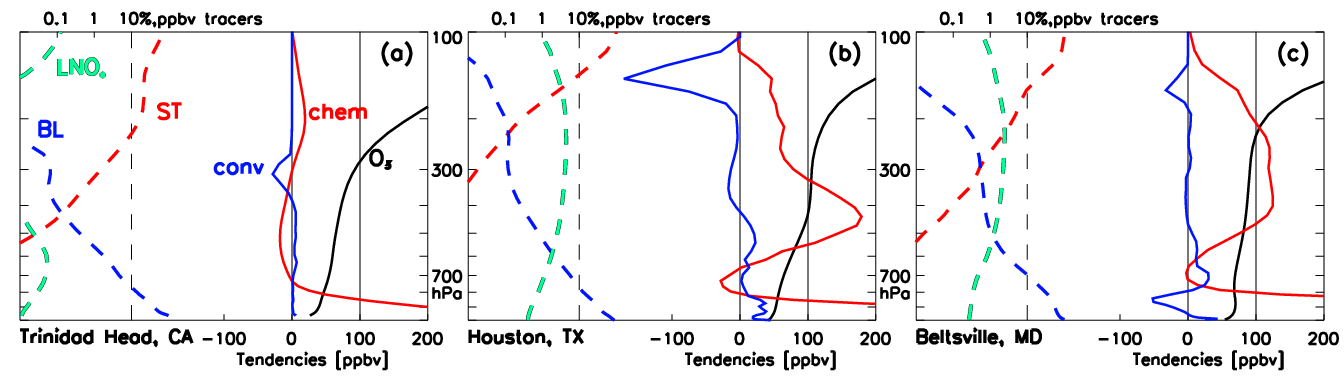
\includegraphics[width=1.0\textwidth]{tendency/vertical.png}
		\caption[Vertical profiles of decaying tracers and tendency diagnostics]{\textbf{Vertical profiles of decaying tracers
		and tendency diagnostics} --- August vertical profiles at ({\bf a}) Trinidata Head, ({\bf b}) Houston,
		and ({\bf c}) Beltsville. Dashed lines are the mean 1-d decaying tracers for BL (blue, \unit{\%}), ST (red, \unit{\%}), and {\lnox} (cyan,
		\unit{ppbv}) according to the values of the top axis. Solid lines are the accumulated chemical tendency diagnostic (red), convective
		tendency diagnostic (blue), and mean ozone profiles in \unit{ppbv} according to the values of the bottom axis. Closest $11\times11$
		grids to the IONS-06 site are selected to compute these profiles.}\vspace{-.3in}
	\end{figure}

Figure~\ref{fig:2006/tendency_vertical} shows the vertical profile of the mean decaying tracers and accumulated
tendencies within 5 grids ($11\times11$) surrounding the
IONS-06 site from August 1st 00\,\unit{UTC} to August 31 00\,\unit{UTC}. The differences between the three locations are again evident. The inflow
region lacks both BL air and {\lnox} in the upper troposphere. Despite comparable ozone level, the accumulated tendency in the upper
troposphere remains low with a maximum of $19.4\pm2.5\,\unit{ppbv}$. Because of the lack of in-situ chemical production, the ozone level remains
low between stratospheric intrusion episodes, allowing the air to remain relatively ``clean'' until reaching Minnesota (Fig.~\ref{fig:2006/o3_300}).
This influx of low-ozone, chemically-``slow'' air mass between each jet stream is therefore responsible in generating the oval-shaped
ozone enhancement that trace the mean circulation in the seasonal average.

At Houston, at the center of the mean-state anticyclone, both the ozone chemical and convective tendencies are substantially higher than Trinidad Head.
At 200\,\unit{hPa}, where Trinidad Head records the peak net upper tropospheric ozone production, Houston records $55.8\pm18.6\,\unit{ppbv}$, about
2.9 times higher. However, this number, as discussed earlier, has been suppressed due to large negative phases of the diurnal cycle. This is due to the
large amount of BL precursor and {\lnox} as indicated by the tracers. Substantial amount of BL precursor is transported into the upper troposphere through
convection, with a mean maximum detrainment height of 145\,\unit{hPa} and a net tendency of $-170\,\unit{ppbv}$ \chem{O_3}, though this may be in part
caused by  a nearby outlier with $-1170\,\unit{ppbv}$\footnote{Such substantial convective tendency is an indication for stationary features such as sea
breeze or orographically triggered convections.} during August. However, the chemical maximum (ignoring BL) occurs in the mid-troposphere at
$437\pm2\,\unit{hPa}$ with a net production of $178\pm51\,\unit{ppbv}$. The position of this peak can be explained by the coincidence of the maximum
level for the prescribed {\lnox} emission based on \citet{Ott:2010lo} and the availability of BL air. As a consequence of production at this level, the mean
ozone VMR exceeds 100\,\unit{ppbv} at 437\,\unit{hPa}. In contrast, without {\lnox}, ozone loss via chemistry is expected at this level as
demonstrated at Trinidad Head.

In the outflow region, though having lower ozone VMRs in the mid-to-upper troposphere compared to Houston, there is a higher net in-situ production of
ozone in the upper troposphere. This can be attributed to having less frequent negative phases that destroy ozone at night. Despite the smaller net
convective tendency, BL tracer is higher than or comparable to the Houston column, indicating that the precursors are advected from elsewhere. An
in-depth analysis of he ozone budget and variability at this location and New England can be found in \citet{Thompson:2007gd,Thompson:2007ov}, which 
utilizes IONS-04, the predecessor of IONS-06.

\subsubsection{Chemical pathways}

The approach above cannot be used to attribute the simulated chemical tendency to the appropriate chemical pathway. Considering the nonlinear
dependency of ozone
production/loss on the atmospheric composition, higher-ordered relation needs to be examined. For urban pollution, the Empirical Kinetic Modeling
Approach (EKMA) has been used to estimate the ozone isopleths in relation to VOC and \chem{NO_x} ratio \citep{Dimitriades:1977fk}. However, this model
suffers several deficiencies, including the lack of dependency on temperature, solar radiance, and transport, all of which can substantially impact the
rates of the presumed ozone steady state. By incorporating simple trajectories and taking into account location and time information, EPA's
OZIPR\footnote{Research-oriented Ozone Isopleth Plotting Package (OZIPP)}model can compute ``city-specific'' EKMA, which is used by
planners to achieve National Ambient Air Quality Standards (NAAQS) compliance and developers to construct research models.

\figuremacroN{tendency/chem_EKMA}{Ozone chemical tendency in relation to \chem{NO_x}}{\label{fig:2006/nox_EKMA}
Ozone chemical tendency in relation to \chem{NO} and \chem{NO_2} chemical tendencies between 15 and 21\,\unit{UTC} in August near Houston, TX
at 200--600\,\unit{hPa} \vspace{-.2in}}

Similar to EKMA, but instead of relating ozone VMR to species VMRs, here we relate ozone to relevant species within the anticyclone
using their chemical tendencies. Figure~\ref{fig:2006/nox_EKMA} shows the net ozone production between each 3-hourly output given
\chem{NO} and \chem{NO_x} chemical tendency during daytime (15--21\,\unit{UTC}) and within 5 model grids from the IONS-06 Houston
launch site at heights with August mean pressure 200--600\,\unit{hPa}. The \chem{NO}+\chem{NO_2} chemical tendency is generally
negative, thus indicating that non-\chem{NO_x} nitrogen species are being produced, e.g. \chem{NO_3}, \chem{HNO_4}, \chem{HONO},
which can explain the strong nocturnal loss phase in ozone. However, this does not guarantee a negative overall \chem{NO_x} tendency
due to \chem{NO} emission from lightning. Finally, ozone production is generally small when the \chem{NO_x} tendency is small (close to the
steady state line), and ozone production occurs when  $\Delta_{chem}\chem{NO}$ is negative while $\Delta_{chem}\chem{NO_2}$ is small.

Since the chemical tendency is fundamentally tied to the chemical mechanism, i.e. the available chemistry set, it is possible to generalize this distribution to other
locations at the same local time\footnote{This requirement guarantees similar photolysis rates ignoring the presence of shadows from deep convective clouds.}
using only a subset of chemical tendency diagnostics. Let $\mathbf{x}$ be a feature vector of length 8, where $x_0=1$ and $x_1\ldots x_5$ be the chemical
tendencies for \chem{CO}, \chem{NO_x}, and \chem{HO_x} in \unit{ppbv/hr}. Chemical tendency for ozone which is designated as $y$. Using a least-square
regression with $L^2$-regularization parameter $\lambda=1$, we fit the following function to the Houston daytime data:
\begin{equation}\label{eqn:chem_ekma}
	y = \mathbf{x}\mathbf{A}\mathbf{x}^T
\end{equation}
where $\mathbf{A}=\{a_{ij}\}_{i,j}$ is a $6\times6$ upper triangular matrix, $\mathbf{x}=(x_0,x_1,\ldots x_5)^T$. Table~\ref{table:2006/ekma_regress}
shows the coefficients of $\mathbf{A}$ from a 100 bootstrap iterations trained on 40.8k (50\%) and tested on 40.8k (50\%) of the data points. The
RMS errors for the regressions from the bootstraps are $0.2954\pm0.0008\,\unit{ppbv/hr}$. Applying the same fitted model to Beltsville gives RMS
errors of $0.2651\pm0.0003$\,\unit{ppbv/hr}.

	\begin{table}[htp!]
	\caption[Quadratic regression on chemical tendencies]{Mean and standard deviations of the coefficient matrix $\mathbf{A}$ in
	Equation~\ref{eqn:chem_ekma}. Insignificant terms where $M_{ij}=\max|\overline{a_{ij}}x_ix_j|<10^{-3}\,\unit{ppbv/hr}$ at Houston
	are shown as $\sim0$, otherwise $\log M_{ij}$ are included in parentheses.}
	\begin{center}
	\begin{tabular}{|c|c|c|c|c|c|c|}\hline
					& 1	& \chem{CO}			& \chem{NO}			&\chem{NO_2}		& \chem{HO}		&\chem{HO_2}			\\ \hline
		1			& 0	& $-0.676\pm0.008$		& $-4.45\pm0.019$		&$-5.83\pm0.030$	& $0.484\pm0.031$	& $-9.33\pm0.147$		\\
					&	& $(0.273)$			& $(0.689)$			& $(0.666)$		& $(-2.86)	$		& $(-0.543)$			\\ \hline
		\chem{CO}	& -	& $-23.2\pm0.265$		& $0.549\pm0.014$		&$-0.206\pm0.048$	& $-1.10\pm0.086$	& $\sim0$				\\
					& 	& $(-0.274)$			& $(0.625)$			& $(-0.398)$		& $(-0.080)$		& $(-3.02)$			\\ \hline
		\chem{NO}	& -	& -					& $1.17\pm0.13$		&$2.87\pm0.22$	& $-2.40\pm0.06$	& $-2.57\pm0.16$		\\
					&	&					& $(-1.32)$			& $(-1.01)$		& $(0.460)$		& $(0.351)$			\\ \hline
		\chem{NO_2} 	& -	& -					& -					&$\sim0$			& $0.668\pm0.075$	& $9.50\pm0.13$		\\
					&	&					&					&				& $(-1.94)$		& $-0.827$			\\ \hline
		\chem{HO}	& -	& -					& -					& -				& $-2.92\pm0.13$	&$\sim0$				\\
					&	&					&					&				& $(0.267)$		&					\\ \hline
		\chem{HO_2}	& -	& -					& -					& -				& -				& $-1.60\pm0.05$		\\
					&	&					&					&				&				& $-1.60$				\\ \hline
	\end{tabular} \label{table:2006/ekma_regress}
	\end{center}
	\end{table}

The model represented by Table~\ref{table:2006/ekma_regress} should be applicable for chemical compositions within or near the domain encompassed by
the data from Houston. Let $M_{ij}=\max_{ij}|\overline{a_{ij}}x_ix_j|$ be the maximum tendency contribution to the net ozone tendency. At Houston, the
largest components are \chem{NO} and \chem{NO_2}, with $\log M_{ij}=0.689$ and 0.666 respectively. Due to the compositions, $M_{ij}$'s may have different
upper bounds at different locations. Applying the same model to Beltsville, $\log M_{ij}=0.833$ and 1.041 respectively. The largest differences, however, are in
the components $\langle\chem{HO},\chem{HO}\rangle$, $\langle\chem{NO},\chem{HO}\rangle$ and $\langle\chem{NO},\chem{HO_2}\rangle$, of which the $\log
M_{ij}$'s evaluate to 0.267, 0.460, 0.351 at Houston but 1.016, 0.748, 0.869 at Beltsville, representing a combined $3.3\times$ maximum contribution to the
variability of ozone production by the interactions between \chem{HO_x} and \chem{NO}. The reason for this difference is not due to changes in chemistry, but
the differences in the domain spanned by $\mathbf{x}$, which effectively selects a subset of the mapped ozone tendency values.

\section{Sensitivity study}\label{sec:2006/sens}

There are numerous variables in the base case simulations that can contribute to the model biases as evaluated in Section~\ref{sec:2006/general}. In
particular, the emission and distribution of lightning-generated \chem{NO_x} {\lnox} has been shown to be a significant component in determining the
atmospheric composition in the free troposphere as represented by CTMs \citep{Labrador:2005uq,Cooper:2009nx,Ott:2010lo}. Thus it is useful to perform
sensitivity simulations to determine the range of variabilities caused by the uncertainties in lightning parameterization.

Other than lightning emission, anthropogenic and biogenic emissions are also crucial in determining the atmospheric composition. While having a lesser
degree of uncertainty and sensitivity compared to {\lnox}, urban developments and policy changes can have substantial impacts on the emission inventory
(Sect.~\ref{ssec:intro/ozone/nox}). As such, sensitivity studies on anthropogenic and biogenic emissions are valuable in determining the calibration
requirements for hypothetical scenarios that correspond to potential changes.

\subsection{Lightning emission}\label{ssec:2006/sens/lnox}

Comparison to NLDN flash counts shows that the current lightning parameterization is producing an order of magnitude higher overall flash rates
(Sect.~\ref{ssec:2006/gen/met}). Two simulations are performed to account for the effect of overpredicting lightning flash rate, as well as to evaluate
the sensitivity of the ozone enhancement to the {\lnox}. These two simulations are identical to the base case simulation in Section~\ref{sec:2006/general}
except with lightning tuning parameter set to $0\times$ and $0.1\times$ to represent a control (no lightning) scenario and tuned-lightning scenario. The
resulting spatial distributions of several species at 300\,\unit{hPa} are shown in Figure~\ref{fig:2006/ltngsens_map}.

\figuremacroW{sens/ltngsens.png}{Upper tropospheric sensitivity to lightning}{\label{fig:2006/ltngsens_map}
Model simulated mean {\bf(a)} \chem{O_3}, {\bf(b)} \chem{CO}, {\bf(c)} \chem{NO_x}, and {\bf(d)} \chem{HO_x} for $0\times$, $0.1\times$, and $1\times$
lightning flash rate at 300\,\unit{hPa} for August. Note that \chem{NO_x} is contoured in the $\log$-scale.}{0.9}

% NOx
\chem{NO_x} is substantially increased above background values ($31.6\pm4.5\,\unit{pptv}$) to $135\pm35\,\unit{pptv}$ with $0.1\times$ lightning and
$1680\pm540\,\unit{pptv}$ with $1\times$ lightning. Modeling the contribution of total \chem{NO_x} VMR by {lnox} as follow:
\begin{equation}\label{eqn:nox+lnox}
	\Delta[\chem{NO_x}] = [\chem{NO_x}]-[\chem{NO_x}]_0 = (1-p)[\chem{LNO_x}]
\end{equation}
where $p$ is the percentage loss of {\lnox} in the atmosphere and $[\chem{NO_x}]_0$ is the no-lightning \chem{NO_x} VMR. For small changes in the
atmospheric composition, $p$ should be constant and thus the addition of \lnox should linearly increase $[\chem{NO_x}]$. Falsely extrapolating this
to $1\times$ flash rate, the expected $[\chem{NO_x}]$ would have been $1070\,\unit{pptv}$. However, because of the decrease in \chem{HO_x}, the
primary reagent converting \chem{NO_x} into reservoir species, in response to {\lnox}, $\partial p/\partial [\chem{NO_x}] < 0$, and thus giving us the
simulated $1680\,\unit{pptv}$, higher than the linearly extrapolated value.

% HO_x
Unlike \chem{NO_x}, \chem{HO_x} is substantially decreased with increasing {\lnox} emission. The initial August mean VMR at 300\,\unit{hPa} without
lightning is $6.94\pm0.38\,\unit{pptv}$. This is above the $\sim$4--5\,\unit{pptv} in the Pacific Northwest and inflow regions. It is slightly decreased
to $6.27\pm0.37\,\unit{pptv}$ with $0.1\times$ lightning, or a 10\% decrease from the $0\times$ scenario. At $1\times$ {\lnox} emission, \chem{HO_x}
is further decreased to $1.80\pm0.59\,\unit{pptv}$, far below the value to the northwest, representing a 71\% drop relative to the $0.1\times$ scenario,
which is larger than that would have been obtained if one ($\sim61\%$) were to extrapolate the initial 10\% decrease with an exponential model.
The lowering \chem{HO_x} with increasing \chem{NO_x} is the results of its interactions with \chem{O_3}, \chem{NO_x}, and \chem{CO} after production
from the \chem{O(^1D)+H_2O}, which is presumably proportionally increasing with the increased level of \chem{O_3}. However, because the VMRs
of all species have been perturbed as the result of {\lnox} emission, it is challenging to describe the new mean \chem{HO_x} with {\lnox} relative to
the control state with $0\times$ lightning.

% CO
Even though \chem{CO+OH\rightarrow CO_2+HO_2} is the only chemical loss pathway for \chem{CO} specified in RADM2 and that \chem{HO_x} is
substantially decreased by a factor of 3.8 from $0\times$ to $1\times$ lightning, \chem{CO} decreases with increasing lightning. Without lightning, the
August mean anticyclone VMR for \chem{CO} is $92.3\pm2.8\,\unit{ppbv}$. This is reduced to $89.8\pm.2.4\,\unit{ppbv}$ with $0.1\times$ lightning
and $85.5\pm2.4\,\unit{ppbv}$ with $1\times$ lightning. The anti-correlation of \chem{CO} with {\lnox} can be described by the dominating effect of
reduced in-situ production of \chem{CO} from \chem{(HCHO,GLY,MGLY)+OH} over increased production from \chem{(OL2,OLT,OLI,ISO)+O_3}.
\footnote{\chem{OL2}=ethene; \chem{OLT}=terminal alkenes; \chem{OLI}=internal alkenes.}

% O3
Finally, \chem{O_3} is increased with increasing {\lnox}, consistent with prior studies on this subject. Perhaps more surprisingly, there is barely
any signs of \chem{NO_x}-titration, which is expected to occur at exceedingly high level of \chem{NO_x}-VOC ratios as observed in polluted urban
environments. The only indication that the model is approaching \chem{NO_x}-titration is the lowering \chem{HO_x}. The \chem{O_3} VMR
is increased from $74.5\pm5.3\,\unit{ppbv}$ to $86.4\pm6.7\,\unit{ppbv}$ ($+16\%$) by adding $0.1\times$ {\lnox}. At $1\times$ lightning, it
is further increased to $101.1\pm6.8\,\unit{ppbv}$, a $26.6\,\unit{ppbv}$ or $36\%$ increase relative to $0\times$ lightning. The reduced sensitivity
to {\lnox} at higher flash rate parameter is consistent with that of \chem{CO}.

There is also a difference in the spin-up time for species in responding to {\lnox} emission due to the lifetime of their respective lifetime in
the atmosphere While the differences in \chem{NO_x} between simulations become apparent within the first day, \chem{HO_x} requires 
two days, which is delayed by a separate spin-up from exchanging between \chem{HO_x} and reservoir species. On the other hand,
\chem{O_3} and \chem{CO} begin to diverge after the fifth day of the simulation when the $Z_{300}$ exceeded 9730\,\unit{m} for the first
time.  However, even after sufficient ``spin-up,'' the differences between simulations can shrink again when air mass with minimal lightning
influence is transported into the region.



%o3:       74.4501      5.28160
%co:       94.2718      2.77095
%NOx:       31.5665      4.48547
%HOx:       6.93762     0.378603

%o3:       86.4036      6.68674			(+11.9) +16%
%co:       89.8467      2.38789			(-4.5)
%NOx:       135.365      34.9208			(+103.4)
%HOx:       6.27117     0.368946		(-0.666)

%o3:       101.067      6.79265			(+14.6)
%co:       85.4519      2.37563			(-4.3)
%NOx:       1678.35      535.866			(+1543)
%HOx:       1.79844     0.585140		(-4.473)

\subsection{Anthropogenic emission}\label{ssec:2006/sens/anthrop}
\subsection{Biogenic emission}\label{ssec:2006/sens/bio}

\section{Conclusions}\label{sec:2006/conslusion}